\documentclass[11pt]{amsbook}

\usepackage{../HBSuerDemir}	% ------------------------


\begin{document}

% ++++++++++++++++++++++++++++++++++++++
\hPage{b2p1/013}
% ++++++++++++++++++++++++++++++++++++++



% =======================================
    \[ \left| a_n - a \right| < \epsilon \quad for  \: all \quad n > N \]
    
    
    \\ a) considering the difference \(A_n - a\), we have
    \[ A_n - a = \frac{a_1 + ... + a_n}{n} - a = \frac{(a_1- a) + ... + (a_n - a)}{n} =\]
    \[ = \quad \frac{(a_1- a) + ... + (a_N - a)}{n} + \frac{(a_{N+1}- a) + ... + (a_n - a)}{n}\]
    \[ \left| A_n - a \right| \leq \frac{\left|a_1- a\right| + ... + \left|a_N - a\right|}{n} + \frac{\left|a_{N+1}- a\right| + ... + \left|a_n - a\right|}{n} = \]
    \[<  \frac{\left|a_1- a\right| + ... + \left|a_N - a\right|}{n} + \frac{(n-N)\epsilon}{n} \]
    
    \\ For sufficiently large n, say for \(N_1 > N\) the first term on the right hand side is less than $\epsilon$, and 
    \[ \left| A_n - a \right| < \epsilon + \frac{(N_1-N)}{n}\epsilon = k\epsilon \]
    
% =======================================
    b) \(G_n = \sqrt[n]{a_1 \quad ... \quad a_n} \Rightarrow  \ln G_n = \frac{\ln a_1 + \quad ... \quad + \ln a_n}{n} \to \ln a\) by \((a) \Rightarrow G_n \to a\).

% =======================================
   \\ \underline{Proof}(5)
   
   a) Applying 4b to \(a_n = (\frac{n+1}{n})^n \to e\), we have
    

% =======================================================
\end{document}  

%==== templates ====

%==== environments ====

%\begin{figure}[htb]
%	\centering
%	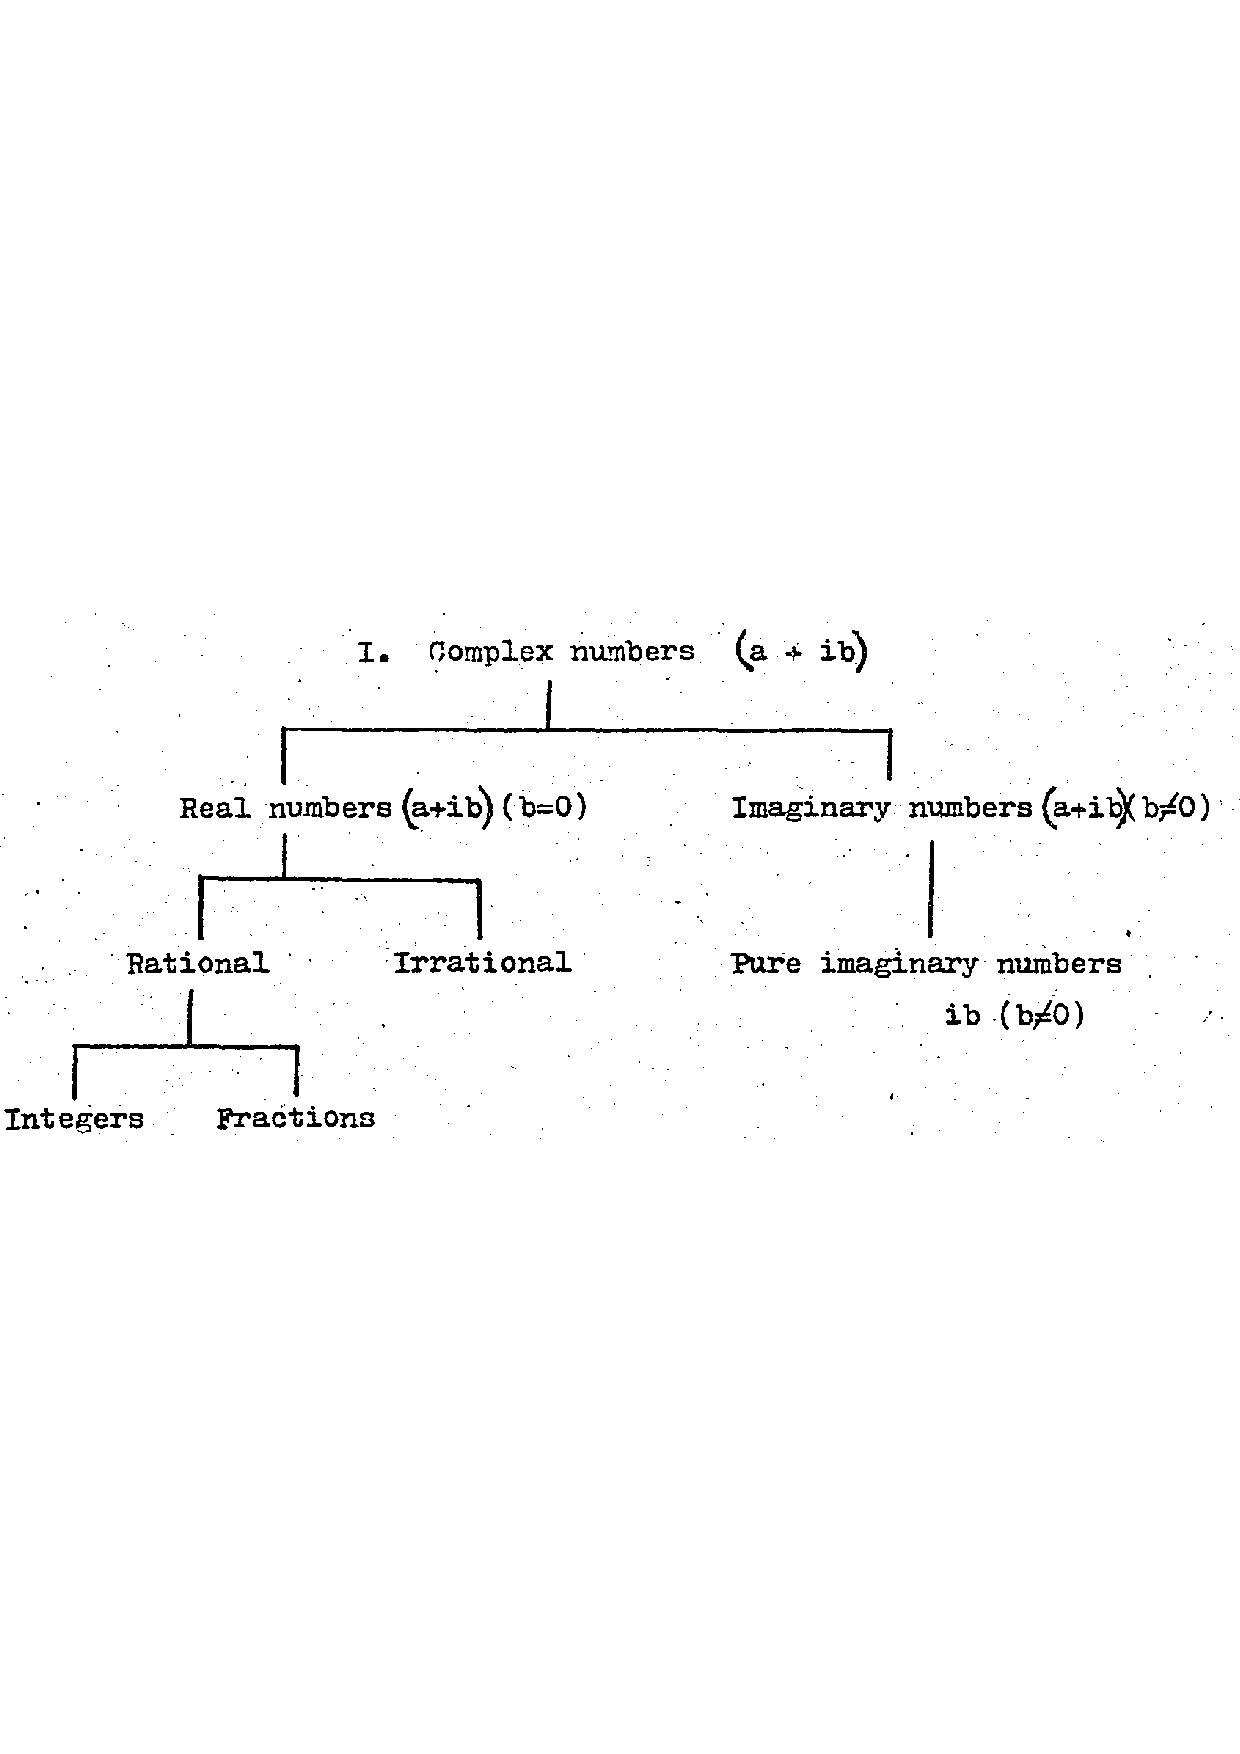
\includegraphics[width=0.9\textwidth]{images/SD-1-1p15A}
%	\caption{Classification of complex numbers}
%	\label{fig:classificationOfComplexNumbersA}
%\end{figure}

%\begin{center}
%\begin{tabular}{cc}
%\end{tabular}
%\end{center}

%\begin{exmp}
%\begin{hSolution}
%\end{hSolution}
%\end{exmp}

%\begin{hEnumerateAlpha}
%\end{hEnumerateAlpha}

%\begin{hEnumerateRoman}
%\end{hEnumerateRoman}

%$
%\begin{bmatrix}
%\end{bmatrix}
%$

%\frac{aaaa}{bbb}
%\frac{a_{n}}{b_{n}}
%\left( aaaa \right)
%\Longrightarrow

%\begin{multicols}{2}
%	bb
%\columnbreak
%	aa
%\end{multicols}
